
\documentclass{beamer}

\usepackage[utf8]{inputenc}
\usepackage[spanish]{babel}

\usepackage{beamerthemesplit}

\usetheme{Warsaw} 

\title{Redes neuronales multicapa}
\subtitle{Castiglione, Karpovsky, Sturla }
\author{Sistemas de Inteligencia Artificial}
\date{3 de Mayo de 2012}

\AtBeginSection[]
{
  \begin{frame}{Tabla de contenidos}
    \tableofcontents[currentsection]
  \end{frame}
}


\begin{document}

\frame{\titlepage}

\section[Outline]{}
\frame{\tableofcontents}

\section{Introducción}
\subsection{El problema}
\begin{frame}{El problema}

\par El problema planteado consiste en la estimación de funciones escalares a partir de un conjunto de puntos que las representan.
\vspace{10px}
\par En nuestor caso particular hemos trabajado con el archivo \textbf{samples7.txt}

\end{frame}

\begin{frame}{Gráfico de la función}

\begin{figure}[H]
\begin{center}
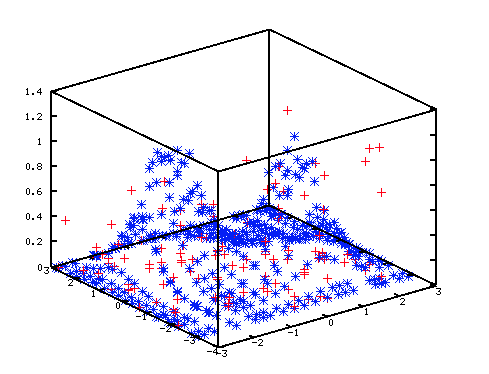
\includegraphics[scale=0.50]{./images/funcion.png}
\label{modelado}
\end{center}
\end{figure}

\end{frame}




\section{Modelado del problema}
\subsection{Representación de la red neuronal}

\begin{frame}{Representación de la red neuronal}
\par Se representó la red neuronal como una matriz de pesos. \\
\begin{itemize}
\item Cada neurona es una columna de pesos.
\item Cada capa de neuronas es una matriz de pesos.
\item La red neuronal, por consiguiente, es un vector de matrices.
\end{itemize}
\end{frame}

\subsection{Funciones de activación}
\begin{frame}
 Se utilizaron dos funciones de activación distintas:
\begin{block}{Sigmoidea exponencial}

\[
  g(h) = \frac{1}{1 + e^{-2 \beta h}} 
\]

Derivada:

\[
  2 \beta g(1-g) 
\]

\end{block}

\begin{block}{Tangente hiperbólica}

\[
  g(x) = tanh(x) 
\]

Derivada:

\[
  \beta g(1-g^2) 
\]

\end{block}

\end{frame}


\subsection{Arquitecturas}

\begin{frame}{Arquitecturas estudiadas}
\begin{itemize}
\item Perceptron simple?
\item Pocas neuronas, pocas capas
\item Muchas neuronas, muchas capas
\item Punto intermedio
\item Conexiones muertas/rotas
\end{itemize}
\end{frame}

\subsection{Cálculo del error}

\subsection{Conjuntos de entrenamiento y testeo}
\begin{frame}{Conjunto de entrenamiento y testeo}
\par Se decidió seguir el consejo de la cátedra y al realizar las pruebas se utilizó un subconjunto de los datos seleccionados al azar para la fase de aprendizaje y el subconjunto restante para testeo.

\begin{itemize}
\item Elección de puntos al azar? Puntos representativos?
\end{itemize}
\end{frame}

\section{Mejoras al algoritmo backpropagation}

\subsection{Eta dinámico}
\begin{frame}{Eta dinámico ($\eta$ adaptativo)}
\begin{itemize}
\item Si el error sube consistenemente incrementar eta aritméticamente: quizás se está siendo muy conservador.
\item Si el error incrementa, reducir $\eta$ exponencialmente.
\end{itemize}
\end{frame}

\subsection{Ruido y momentum}
\begin{frame}{Momentum}
\[w_{ij}(t+1)= - \frac{\partial E}{\partial w{ij}} + \alpha w(t)\]
\par Cambios dependen de cambios anteriores. Idea de dirección general del error. 
\par Olvido exponencial de cambios anteriores.
\par Se aplica a cada batch / lote
\end{frame}

\begin{frame}{Ruido}
\par \textbf{Idea:} Escape del mínimo local.\\
\par Robustez de la red neuronal: debería poder soportar ruido.
\end{frame}

\section{Resultados}

\begin{frame}{Resultados 1}
\begin{figure}[H]
\begin{center}
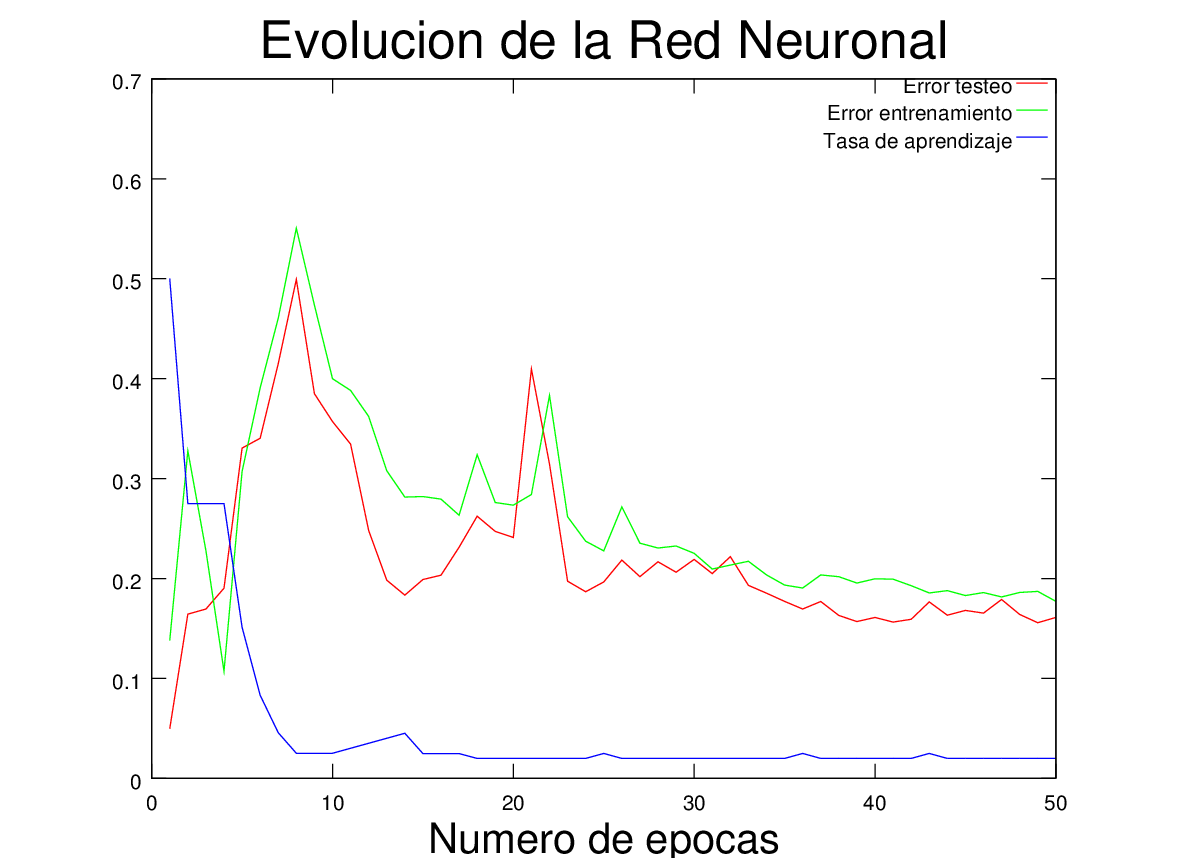
\includegraphics[scale=0.38]{../images/6.png}
\label{modelado}
\end{center}
\end{figure}

\begin{center}
\par Figura 1: Arq [200 100], eta adaptativo, tangente hiperbólica
\end{center}
\end{frame}

\begin{frame}{Resultados 2}
\begin{figure}[H]
\begin{center}
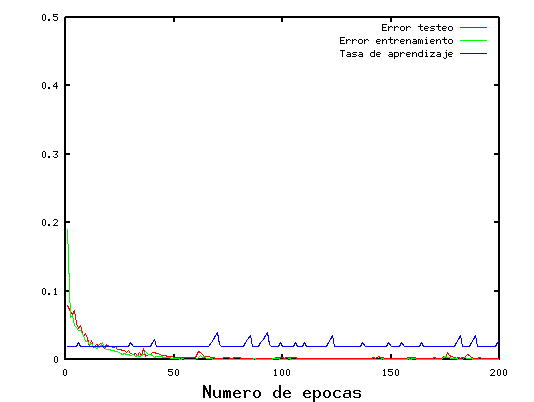
\includegraphics[scale=0.50]{../images/nice.png}
\label{modelado}
\end{center}
\end{figure}

\begin{center}
\par Figura 2: Arq [50 30] 200 epocas, tangente hiperbólica.
\end{center}
\end{frame}

\begin{frame}{Resultados 3}
\begin{figure}[H]
\begin{center}
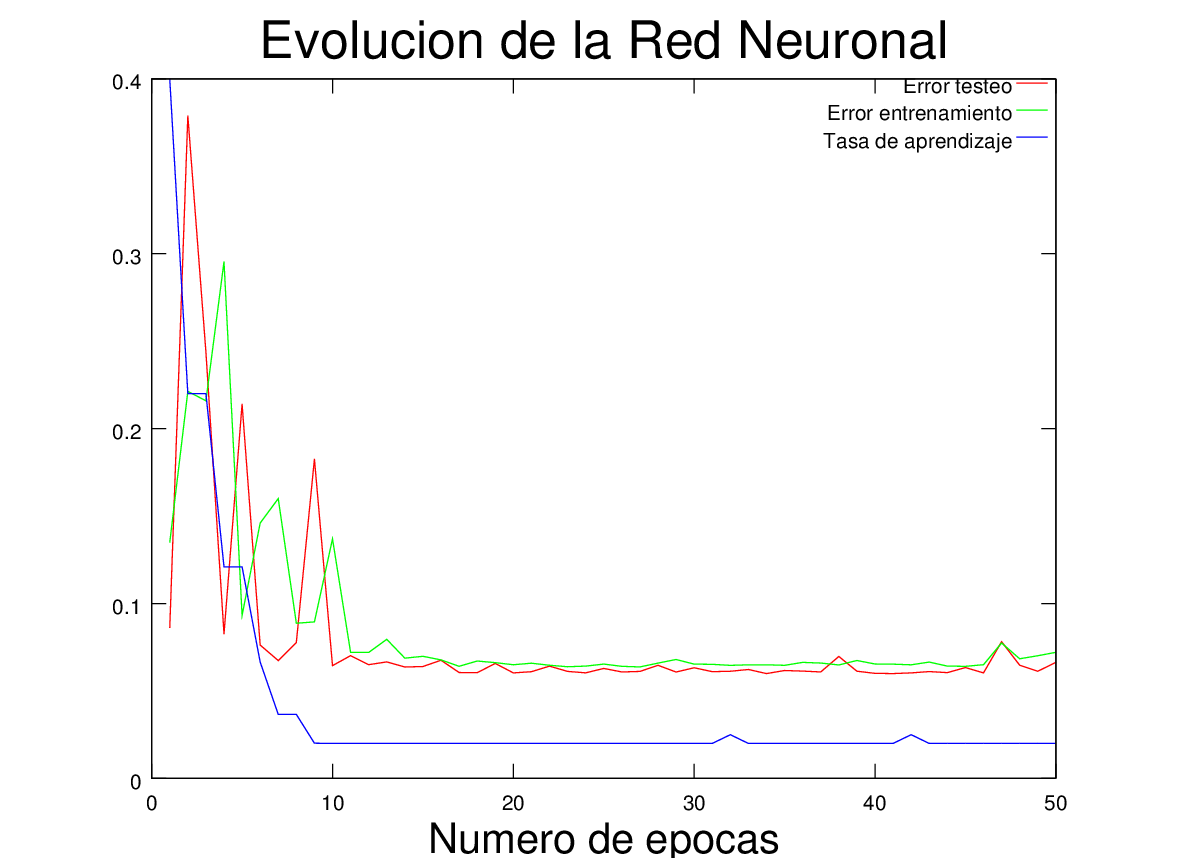
\includegraphics[scale=0.38]{../images/9.png}
\label{modelado}
\end{center}
\end{figure}

\begin{center}
\par Figura 3: Arq [4 4] 200 épocas eta adaptativo, tanh.
\end{center}
\end{frame}

\section{Conclusiones}
\begin{frame}{Conclusión}

\begin{itemize}
\item Incrementar la cantidad de neuronas arbitrariamente no necesariamente 
implica mejoras en cuanto al error (puede llevar a malas generalizaciones y tiempo de más 
hasta alcanzar el error desdeado).\\
\item No existe tal cosa como una mejor arquitectura o parámetros óptimos. Estos seguramente dependan 
el problema que se está analizando.\\
\end{itemize}

\end{frame}

\begin{frame}{Conclusión cont.}
\begin{itemize}

\item Momentum no siempre puede acelerar la convergencia.\\
\item La función de activación \textit{exponencial} es más propensa a atascarse en mínimos.\\
\item Tomar pocos puntos puede ser una muestra poco representativa, y por lo tanto, puede haber mala generalización.\\
\end{itemize}
\end{frame}

\end{document}
